\documentclass{article}  % Define la clase del documento.

% Paquetes de idioma y codificación
\usepackage[utf8]{inputenc}
\usepackage[T1]{fontenc}
\usepackage[spanish]{babel}  % Ajusta el idioma del documento a español.
\usepackage{tabularx}  % Permite la creación de tablas con ancho ajustable.

% Paquete de geometría para configurar márgenes y tamaño de papel
\usepackage[letterpaper, margin=3cm]{geometry}
\usepackage{caption}

% Paquetes de tipografía
\usepackage{mathptmx}    % Usa Times New Roman como fuente.
\usepackage{microtype}   % Mejora la justificación del texto.

% Paquetes para manejo de colores y gráficos
\usepackage{xcolor}      % Define y utiliza colores.
\usepackage{graphicx}    % Permite la inserción de imágenes.
\usepackage{tikz}        % Creación de gráficos vectoriales.

% Configuración de enlaces y referencias cruzadas
\usepackage{hyperref}
\hypersetup{
    colorlinks   = true,
    linkcolor    = darkblue,
    citecolor    = black,
    filecolor    = blue,
    urlcolor     = blue
}

\usepackage{media9} % Permite la inserción de multimedia.

% Paquetes para la mejora visual de tablas y figuras
\usepackage{booktabs}    % Para tablas de alta calidad.
\usepackage{float}       % Controla la posición de figuras y tablas.

% Paquete para la personalización de códigos fuente
\usepackage{listings}
\lstset{
    literate=
    {á}{{\'a}}1 {é}{{\'e}}1 {í}{{\'i}}1 {ó}{{\'o}}1 {ú}{{\'u}}1
    {Á}{{\'A}}1 {É}{{\'E}}1 {Í}{{\'I}}1 {Ó}{{\'O}}1 {Ú}{{\'U}}1
    {ñ}{{\~n}}1 {Ñ}{{\~N}}1 {ü}{{\"u}}1 {Ü}{{\"U}}1,
    backgroundcolor=\color{backcolour},
    commentstyle=\color{codegreen},
    keywordstyle=\color{codepurple},
    numberstyle=\tiny\color{codegray},
    stringstyle=\color{red},
    basicstyle=\ttfamily\small,
    breakatwhitespace=false,
    breaklines=true,
    captionpos=b,
    keepspaces=true,
    numbers=left,
    numbersep=5pt,
    showspaces=false,
    showstringspaces=false,
    showtabs=false,
    tabsize=2,
    language=TeX,
    morecomment=[l]\#,
    frame=single,
    rulecolor=\color{black}
}

% Definición de colores al estilo Visual Studio Code
\definecolor{darkblue}{rgb}{0.0, 0.0, 0.55}  % Enlaces
\definecolor{codegreen}{rgb}{0.25, 0.49, 0.48}  % Comentarios
\definecolor{codegray}{rgb}{0.5, 0.5, 0.5}  % Números y anotaciones
\definecolor{codepurple}{rgb}{0.58, 0, 0.82}  % Palabras clave
\definecolor{backcolour}{rgb}{0.95, 0.95, 0.92}  % Fondo de código

% Configuraciones de párrafo y matemáticas
\usepackage{amsmath}
\usepackage{parskip}    % Espaciado entre párrafos.
\usepackage{ragged2e}   % Justificación mejorada.

% Configuración de secciones y encabezados
\usepackage{titlesec}
\titleclass{\part}{top}
\titleformat{\part}[display]
  {\normalfont\huge\bfseries\centering}{\thepart}{40pt}{\Huge}
\titlespacing*{\part}{0pt}{-60pt}{10pt}
\titleformat{\part}
  {\normalfont\huge\bfseries}{}{0pt}{}
\titleformat{\part}[display]
  {\normalfont\huge\bfseries}{}{0pt}{}
  [\thispagestyle{fancy}]

% Encabezado y pie de página
\usepackage{fancyhdr}
\pagestyle{fancy}
\fancyhf{}
\fancyhead[L]{\raisebox{0.20cm}{\textbf{EPI}}}
\fancyhead[R]{\raisebox{0.1cm}{
\includegraphics[width=0.25\linewidth]{LOGO_UNIVERSIDAD.jpg}}}
\fancyhead[C]{\rule{\textwidth}{0.6pt}}
\fancyfoot[C]{\rule{\textwidth}{0.6pt}}
\fancyfoot[R]{\raisebox{-1.5\baselineskip}{\thepage}}
\renewcommand{\headrulewidth}{0pt}
\renewcommand{\footrulewidth}{0pt}

% Geometría avanzada
\geometry{
  top=3.5cm,
  bottom=2.5cm,
  headheight=2.5cm
}

% Bibliografía
\usepackage{natbib}
\bibliographystyle{unsrtnat}

\begin{document}

%---------------------------------------- PORTADA ----------------------------------------
\begin{titlepage}
\newcommand{\HRule}{\rule{\linewidth}{0.5mm}} 
\center

\includegraphics[width=10cm]{LOGO_UNIVERSIDAD.jpg}\\
\vspace{3cm}
\HRule \\[0.4cm]
{ \huge \bfseries Prueba 2}\\[0.4cm]
{ \huge \bfseries EPI}\\[0.4cm]
\HRule \\[1.5cm]
\vspace{4.5cm}
\begin{flushright}
    \vspace{0.8cm}
    \textbf{Alumnos:} \\
    Lukas Wolff Casanova\\
\end{flushright}
\vspace{1cm}
{\large \textbf{\today}}\\[2cm]
\end{titlepage}



\newpage
\setcounter{page}{1}

%---------------------------------------- CONTENIDO ----------------------------------------
\section{Target Value Design (TVD)}

Metodo que se ideo con el objetivo de conducir el diseño y construccion de un proyecto
hacia el \textbf{logro de los objetivos}

Se busca hacer una adatacion del \textbf{target costing} 

Las diferencias entre el diseño convencional y el TVD son:

\begin{table}[h!]
\centering
\begin{tabular}{|p{6.5cm}|p{6.5cm}|}
\hline
\textbf{TVD} & \textbf{Práctica tradicional} \\
\hline
Ciclo de diseño – estimación – rediseño & Ciclo de diseño – estimación – retrabajo \\
\hline
Se elabora primero un estimado y entonces el diseño es realizado alineándose con el estimado. & El diseño multidisciplinario es dibujado y entonces se hace el estimado en función de él. \\
\hline
El diseño se basa solo en lo que se puede construir. & Es necesaria una evaluación del diseño respecto a constructabilidad. \\
\hline
Todos los diseñadores se involucran desde el diseño inicial. & El arquitecto diseña, entonces otros involucrados basan su trabajo en el proyecto de arquitecto. \\
\hline
El costo objetivo nunca debe ser excedido. & El costo del proyecto excede lo que el cliente puede pagar por él. \\
\hline
\end{tabular}
\caption{Comparación entre TVD y práctica tradicional}
\end{table}

Ahora, para poder llevar a cabo el TVD, se deben cumplir los siguientes aspectos:

\begin{itemize}
    \item Integracion Temprana
    \item Compartir Riesgos y Recomensas
    \item Tener Objetivos Alineados
    \item Diseño Concurrente, compartir el conocimiento sobre costos y experiencias.
\end{itemize}

\begin{figure}[H]
\centering
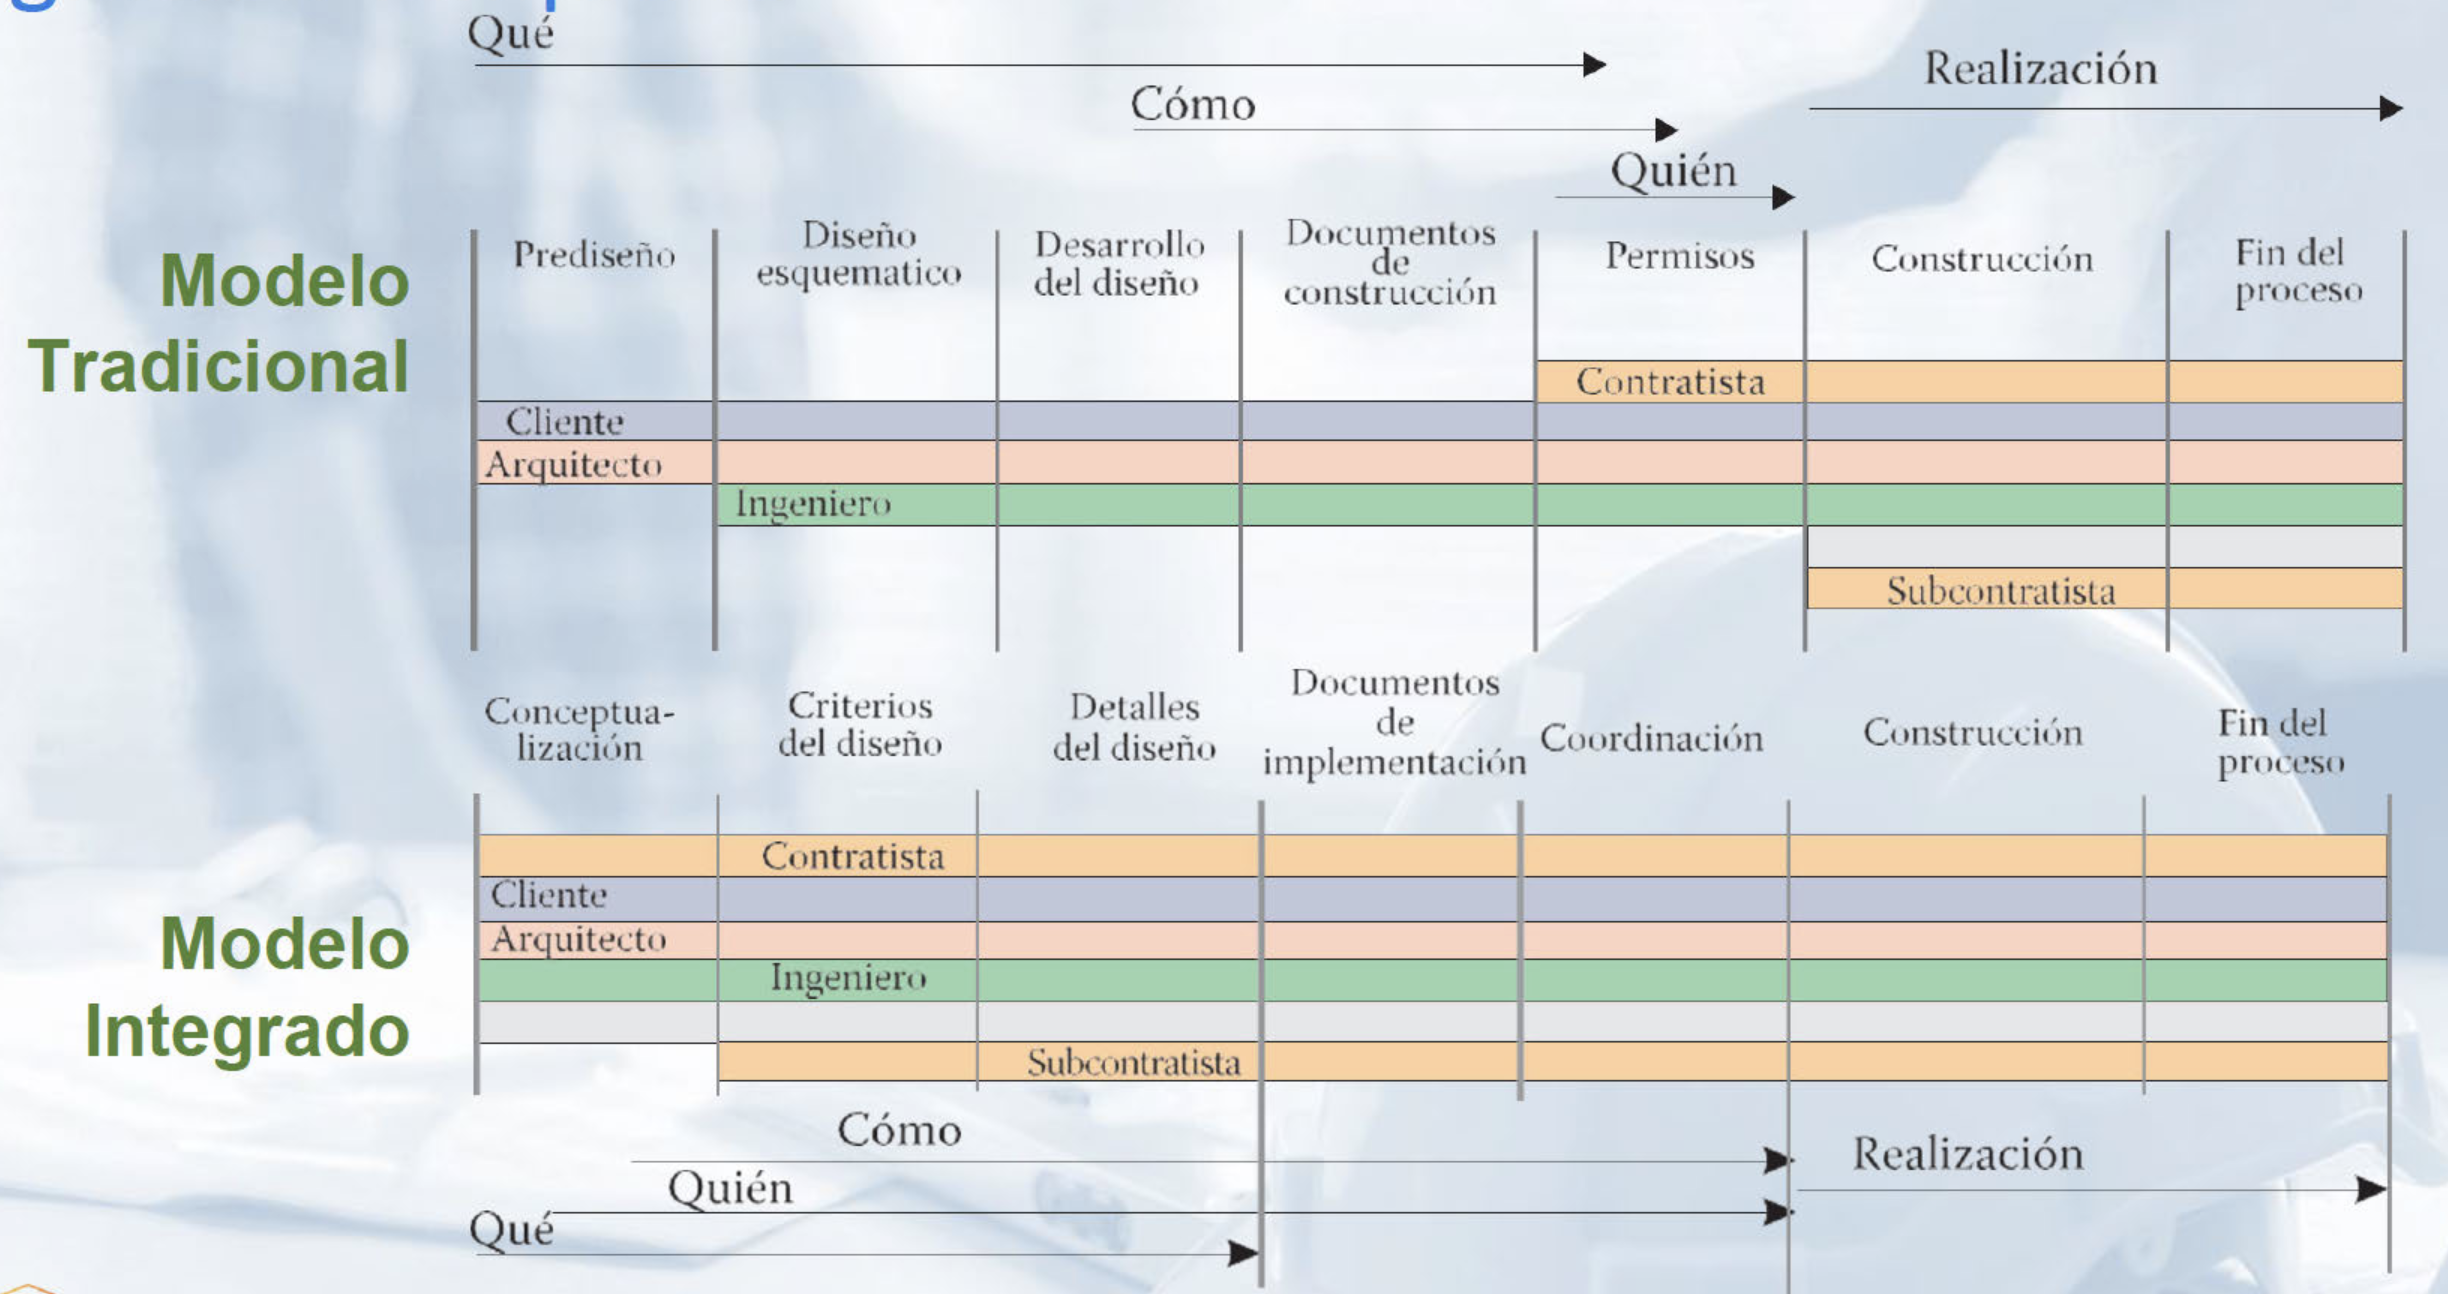
\includegraphics[width=0.8\textwidth]{IMAGENES/TVD.png}
\caption{Proceso de TVD}
\label{fig:tvd}
\end{figure}

Los pasos a ejecutar son:

\begin{itemize}
    \item Definir el costo objetivo para el proyecto
    \item Trabajar estructuradamente
    \item Colaboracion
    \item Set-Based Design
    \item Collocation
\end{itemize}

Ahora bien, algunas buenas practicas a seguir dentro de TVD son:

\begin{itemize}
    \item Comprometerse con el cliente para \textbf{establecer valor objetivo}
    \item Guiar los esfuerzos de diseño hacia el \textbf{aprendizaje y la innovación}
    \item \textbf{Diseñar} en relación con el \textbf{presupuesto y el valor objetivo} del cliente
    \item Planear \textbf{colaborativamente}
    \item Diseñar simultáneamente el \textbf{producto y el proceso}
    \item Diseñar y planear con base en el \textbf{cliente} que utilizará el producto
    \item Trabajar en \textbf{pequeños grupos} multidisciplinarios
    \item Trabajar en un “Big room”. \textbf{Co-location}
    \item Realizar \textbf{retrospectivas} a lo largo del proceso
\end{itemize}

\subsection{Como trabajar en TVD}

De esta forma, se ontiene lo siguiente:


\noindent En lugar de diseñar aisladamente y posteriormente reunirse para revisiones y decisiones de grupo, \textbf{colaboración} 
\[
\Rightarrow \text{Trabajar en equipo para definir los inconvenientes y decisiones y luego diseñar conforme a esas decisiones}
\]

\noindent En lugar de evaluar la constructabilidad del diseño, \textbf{estructura de trabajo}
\[
\Rightarrow \text{Diseñar lo que es construible}
\]

\noindent En lugar de trabajar solos en cuartos separados, \textbf{co-locación}
\[
\Rightarrow \text{Trabajar en parejas o en grupos más grandes, cara a cara}
\]

\noindent En lugar de estimar con base en un diseño detallado, \textbf{costo objetivo}
\[
\Rightarrow \text{Diseñar con base en un estimado detallado}
\]

\noindent En lugar de tomar decisiones que reduzcan las posibilidades para proceder con el diseño, \textbf{Set Based Design}
\[
\Rightarrow \text{Mantener conjuntos de decisiones abiertos a lo largo del proceso de diseño}
\]

\subsection{Beneficios del TVD}

\begin{itemize}
    \item Posicionamiento hasta un 15\% por debajo del precio de mercado
    \item Reducción de costos sin comprometer la calidad, el cronograma o el alcance del proyecto
    \item Reducción de tiempos de ejecución
    \item Buenas relaciones y ausencia de conflictos
    \item Ausencia de reclamos
\end{itemize}

\section{Integrated Project Delivery (IPD)}

\textbf{Claridad} implica:

\begin{itemize}
    \item Conocer cuales son las reglas
    \item Conocer que es ganar
\end{itemize}

\textbf{Alineamineto} implica:

\begin{itemize}
    \item Mismas reglas
    \item Mismas ganancias
\end{itemize}

El IPD es la metodologia que \textbf{Alinea Colaborativamente} a las personas, a los sistemas y los procesos del negocio, para \textbf{Aprovechar}
los talentos de los participantes, asi pueden \textbf{optimizar el proyecto} reduciendo el valor 

De esta forma, el IPD se ve como:

\begin{figure}[H]
\centering
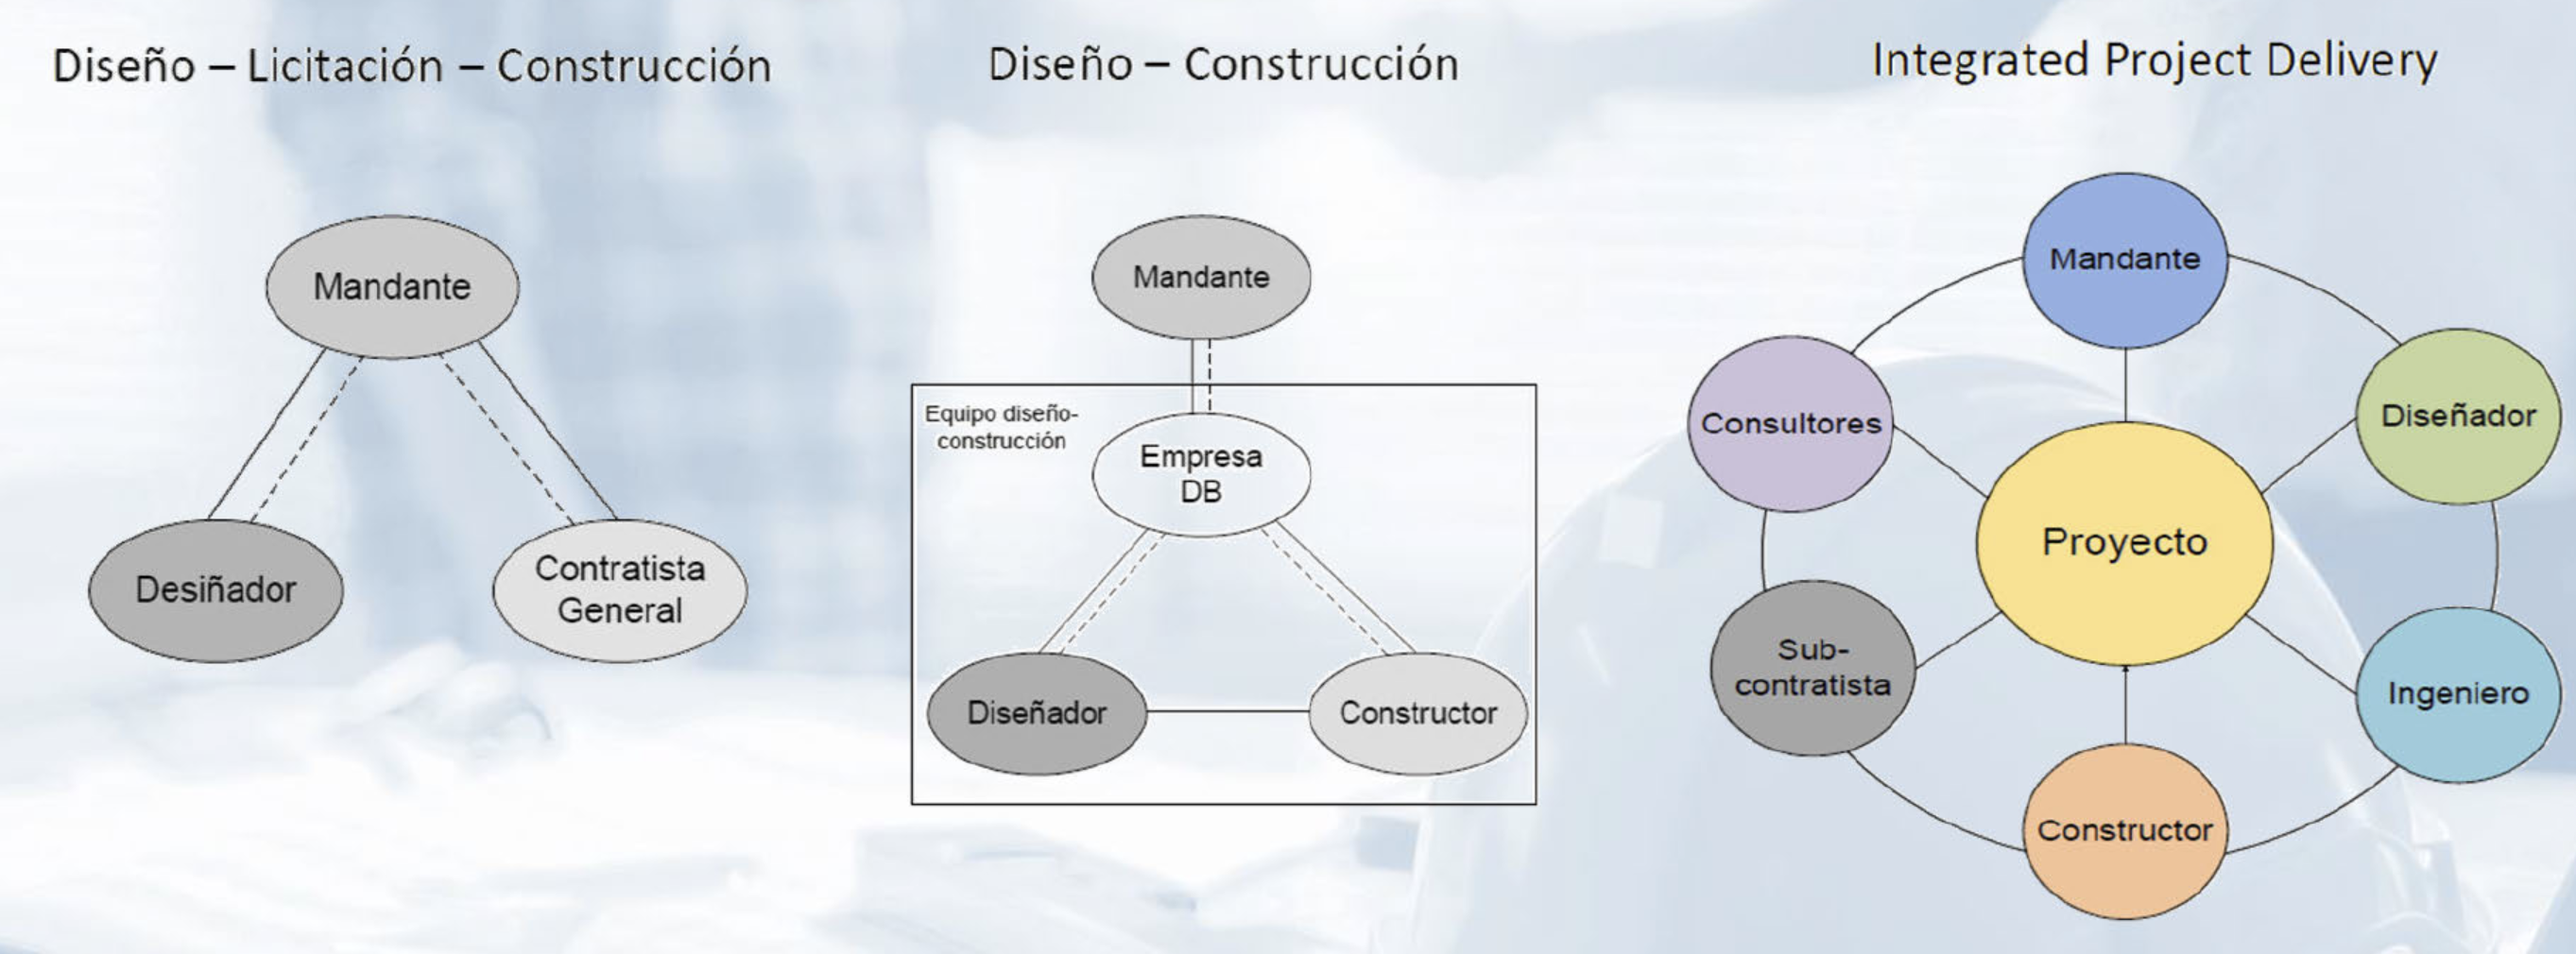
\includegraphics[width=0.8\textwidth]{IMAGENES/IPD.png}
\caption{Proceso de IPD}
\label{fig:ipd}
\end{figure}

De esta forma:

\begin{itemize}
    \item Se basa principalmente en la colaboración y la confianza.
    \item Genera buenos resultados siempre y cuando las personas se respeten mutuamente.
    \item Se centran en obtener buenos resultados para el proyecto y no se desvíen en lograr metas individuales.
\end{itemize}

Donde sus principios son:

\begin{itemize}
    \item Respeto mutuo y confianza
    \item Beneficio mutuo y recompensa
    \item Innovación colaborativa y toma de decisiones
    \item Definición temprana de objetivos
    \item Planificación intensificada
    \item Comunicación abierta
    \item Tecnología apropiada
    \item Organización y liderazgo
\end{itemize}

Y las etapas principales son:

\begin{itemize}
    \item Entrenamiento inicial: Metodología de gestión integrada de proyectos
    \item Validación y socialización de los principios y condiciones de satisfacción del proyecto
    \item Estructuración y definición de roles y responsabilidad del equipo participante, además del análisis y elección de metodologías y recursos a utilizar
    \item Aplicación de metodología y herramienta TVD
    \item Sustento legal que deberá ser definido y estructurado para llevar a cabo el proyecto, marcado por la colaboración y la innovación
\end{itemize}

Y los contratos relacionales son:

\begin{itemize}
    \item Ambiente de confianza, comunicación abierta y participación
    \item Cultura corporativa
    \item Trabajo colaborativo y reciprocidad
    \item Relaciones de largo plazo
\end{itemize}

\section{Metodologia Lean Construction}

\begin{figure}[H]
\centering
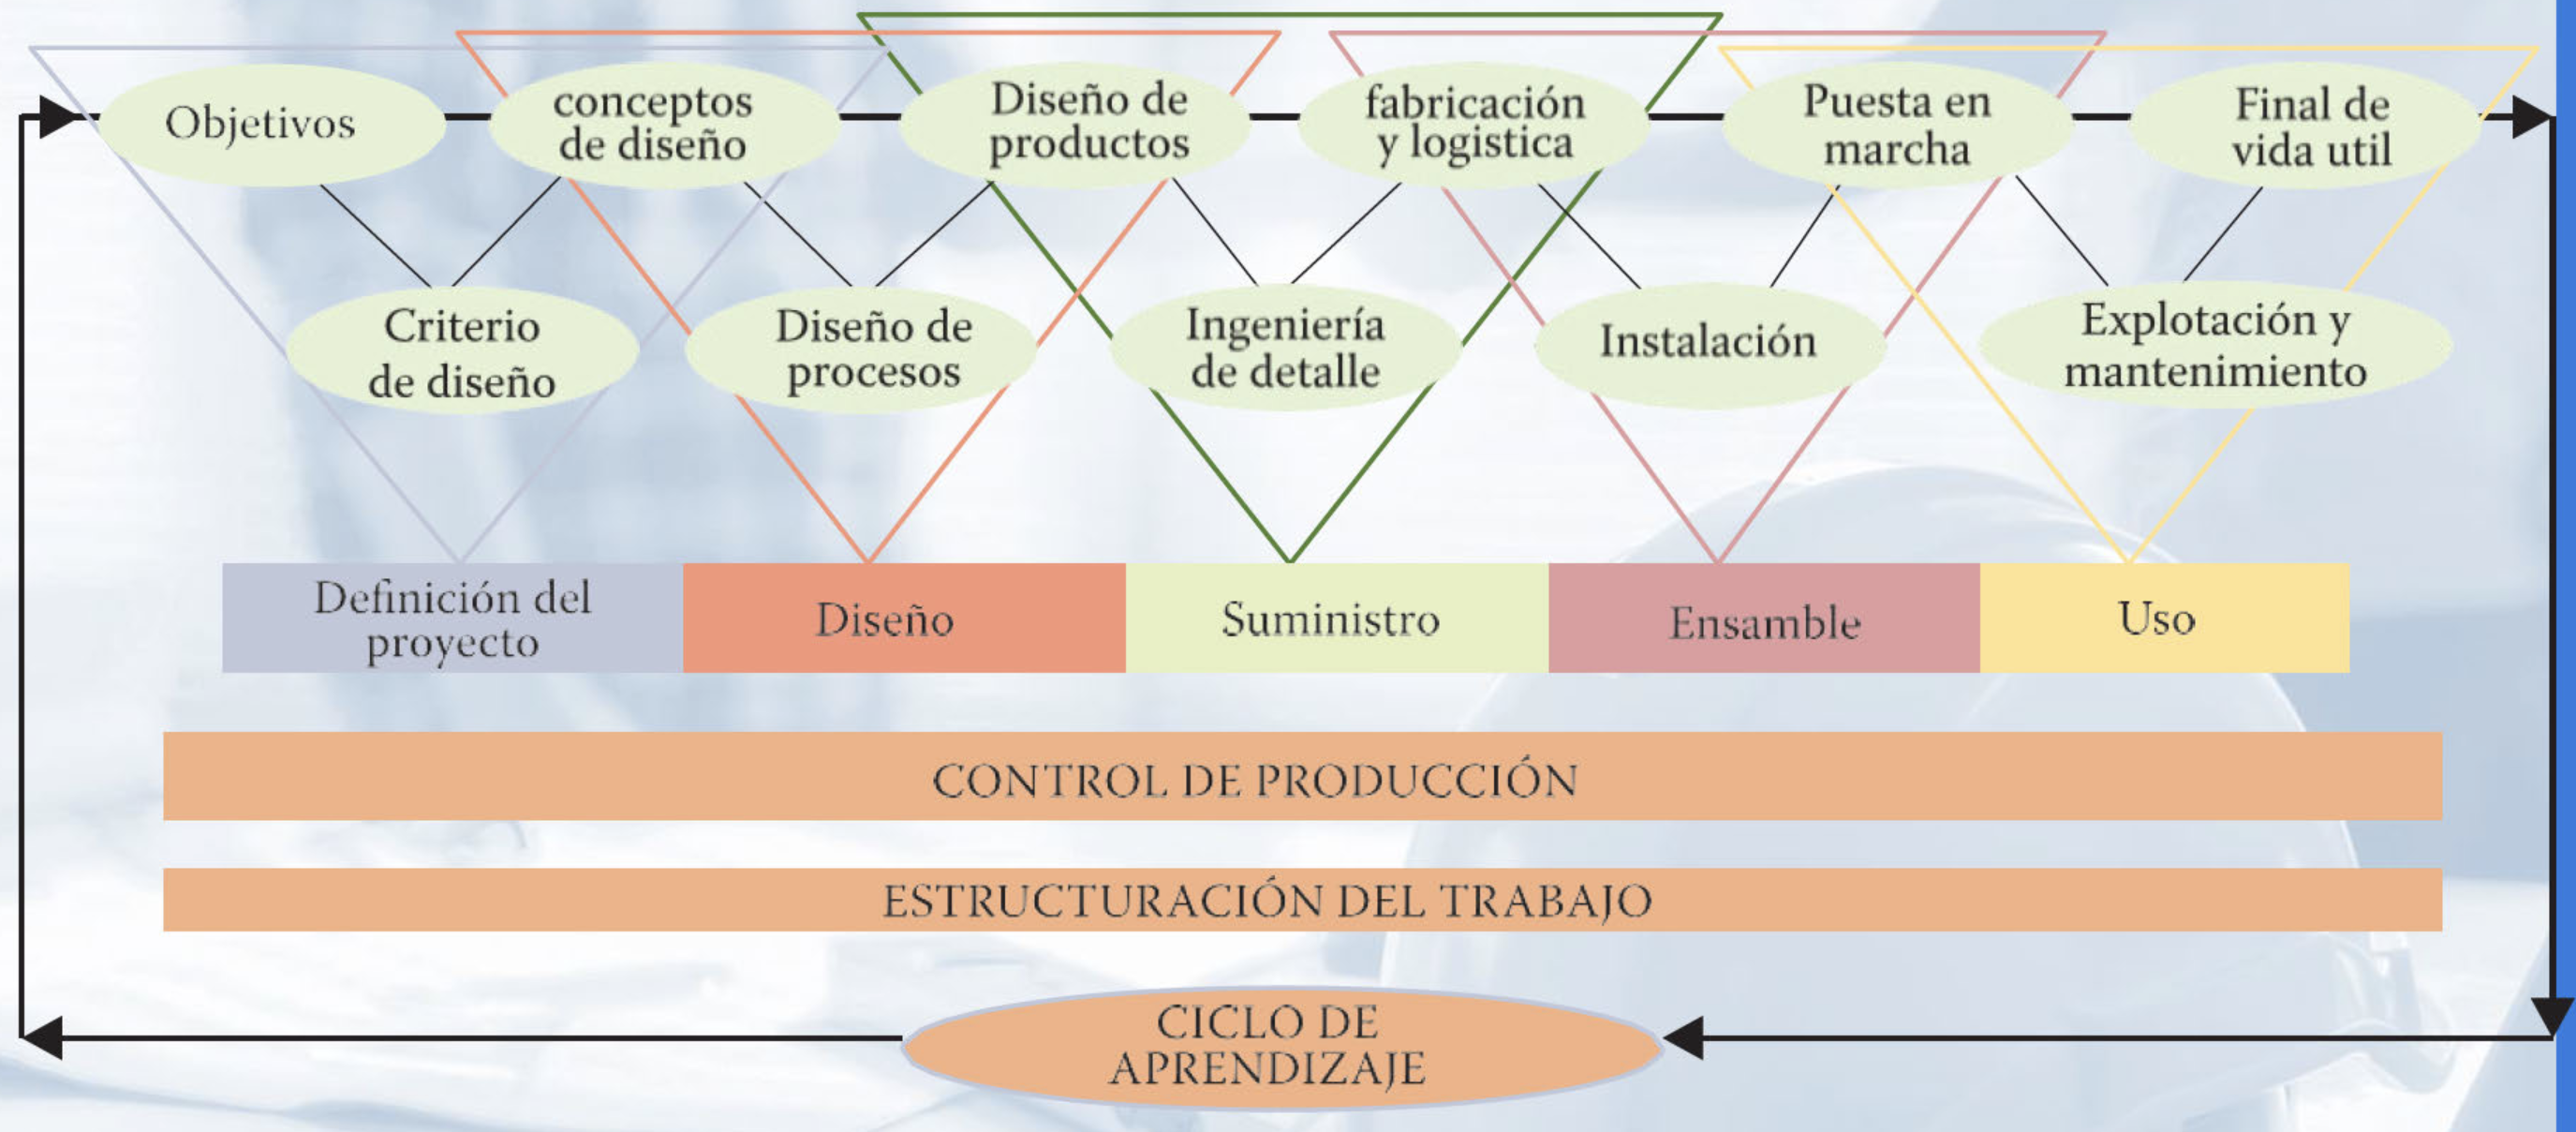
\includegraphics[width=0.9\textwidth]{IMAGENES/LEAN.png}
\caption{Proceso de Lean Construction}
\label{fig:lean}
\end{figure}



\end{document}
